\begin{center}
\textbf{Заключение}
\end{center}

В результате выполнения курсового проекта проведен общетехнический
анализ проектируемого устройства, который включает: анализ исходных данных, описание принципа работы анализируемого устройства, анализ электрической принципиальной схемы устройства, определение параметров воздействующих дестабилизирующих факторов и протекающих физических процес-
лсов для последующего моделирования.

Проведено моделирование физических процессов, воздействующих на
устройство, а именно: обоснование выбора прикладного программного обеспечения для моделирования физических процессов, разработан план моделирования физических процессов, разработана методика построения трехмерной модели исследуемого устройства, проведено моделирование механических
процессов, протекающих в электронном модуле и устройстве в целом, и проведено моделирование тепловых процессов, протекающих в электронном модуле и устройстве в целом.
Основываясь на вышеперечисленном, был проведен анализ полученных
результатов, а также дана краткая оценка.

Таким образом была предпринята попытка реализовать все поставленные цели и задачи на курсовой проект. Однако с уверенностью можно заключить, что эта попытка не была удачной. Большую роль сыграли проблемы с экспортом модели трехмерной модели, случившиеся в результате перехода на другую систему автоматизированного проектирования печатной платы.

Остается только сделать выводы и не допускать ошибок, подобных допущенным при выполнении данного курсового проекта.
  \newpage



% \bibligoraphystyle{5sem}
% \renewcommand{\bibsection}{{Cписок использованных источников}}
\renewcommand{\refname}{\textbf{Cписок использованных источников}}
\DeclareFieldFormat{url}{Режим доступа\addcolon\space\url{#1}}
\DeclareFieldFormat{title}{{#1}}
\DeclareFieldFormat{labelnumberwidth}{[{#1}]\adddot  }
\printbibliography

\newpage
\begin{center}
\textbf{Приложение А}\\
\textbf{Обязательное}\\
\textbf{Параметры компонентов}
\end{center}

Техническое описание ПП:
\begin{enumerate}[label={\arabic*.}]
\item Соотношение сторон 1:1.
\item Габариты ПП 75 на 75 мм.
\item Толщина ПП 0,8 мм.
\end{enumerate}

Данные необходимые для тепловго анализа:
\begin{enumerate}[label={\arabic*.}]
\item Температура окружающей среды 315 К.
\item Коэффициент конвекции — 25 Вт/К * м².
\end{enumerate}

\newpage


\begin{center}
\textbf{Приложение Б}\\
\textbf{Обязательное}\\
\textbf{Отчет о проверке на заимствования в системе «Антиплагиат»}

\begin{figure}[H]
  \centering
  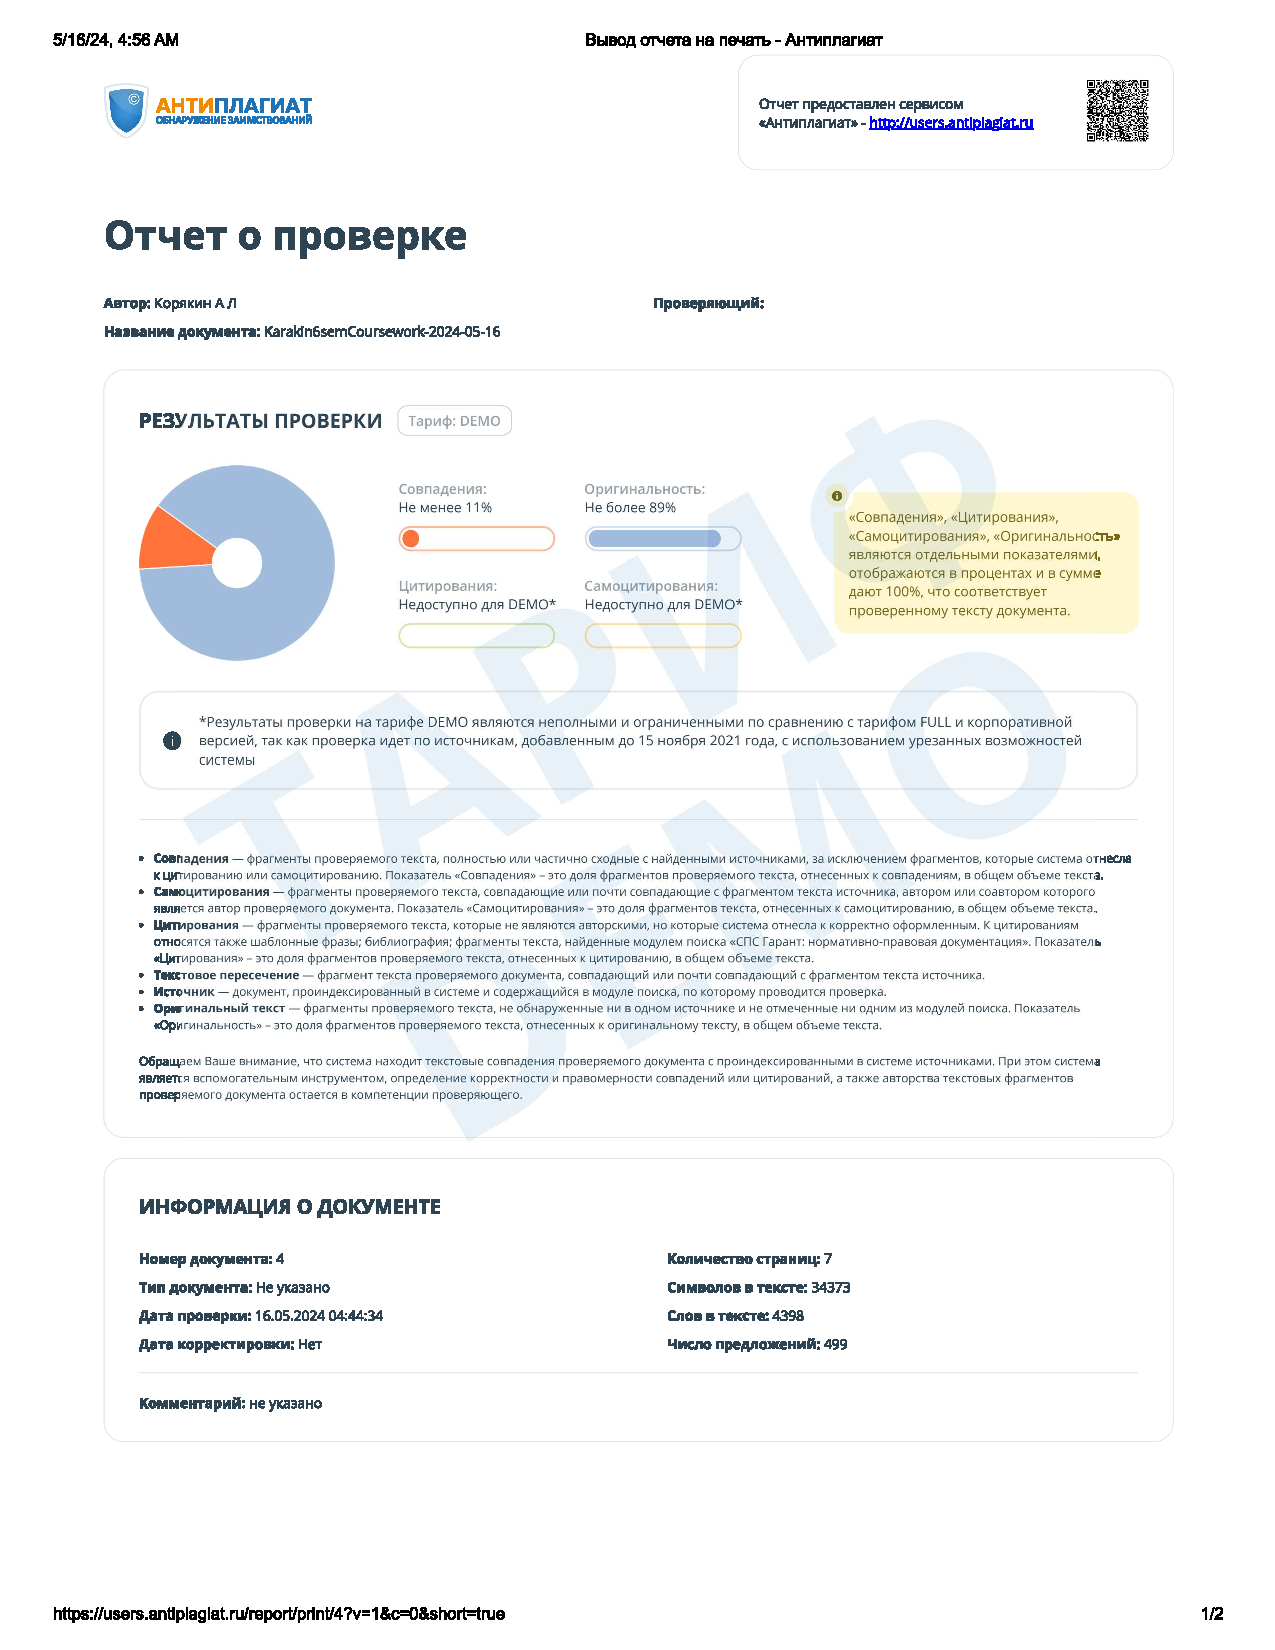
\includegraphics[scale=0.7]{../img/antiplagiat.pdf}
  \caption{Результат проверки на заимстования в системе «Антиплагиат»}
\end{figure}
\end{center}